\documentclass{article}
\usepackage[thmmarks, framed]{ntheorem} % ntueorem must come before amsmath, or the cross-reference will not be working
\usepackage[utf8]{inputenc}
\usepackage{graphicx}
\usepackage{booktabs}
\usepackage[a4paper, portrait, margin=1in]{geometry}
\usepackage{amsmath}
\usepackage{amsfonts}
\usepackage{mathtools}
\usepackage{physics}
\usepackage{siunitx}
\usepackage{xcolor}
\usepackage{lmodern} % in conjugate with the fontenc package to prevent pixelisation of output
\usepackage[T1]{fontenc} % to produce the ``dbar'' in thermo
% needed for framed theorems
\usepackage{framed} % or, "mdframed"
%
\usepackage{bm}
\newtheorem{theorem}{Theorem} 
\newframedtheorem{frm-thm}{Theorem} %needed for framed theorems 
\theorembodyfont{\upshape}
\newframedtheorem{frm-res}{Result}
\theorembodyfont{\upshape}
\newframedtheorem{frm-def}{Definition}
\theoremstyle{nonumberplain} 
\theoremheaderfont{\itshape}
\theorembodyfont{\normalfont}
\theoremsymbol{\ensuremath{\square}}
\newtheorem{proof}{Proof}
\title{NST IB Physics A: Introduction to Condensed Matter Physics}
\date{Easter, 2023}
\author{Yu Lu}
\begin{document}
\maketitle 
\tableofcontents
\section{Lattices and reciprocal lattices}
A crystal can be regarded as convolution of atoms on a lattice of delta functions $\Lambda.$ With a choice of three linearly independent basis vectors $\mathbf{a}, \mathbf{b}, \mathbf{c},$ any lattice vector can be written as
\[
    \mathbf{r} = u \mathbf{a}  + v \mathbf{b} + w \mathbf{c} = [uvw]. 
\]
We are mostly interested in cubic P, I, and F lattices. In a cubic system, there might be equivalent directions due to symmetry. For example, $<100>$ denotes any edge of a cube. 

All lattice points are identical, and we divide the lattice into unit cells. A conventional is the easiest to work with, but it can contain more than one lattice point. Alternatively, a primitive unit cell only has one unit cell, but may not reflect the symmetry of the lattice explicitly. 

We are interested in functions with translational invariance $f(\mathbf{x} ) = f(\mathbf{x} + \mathbf{r}),$ and the lattice of $k$ vectors needed to form a Fourier series of $f$ is the reciprocal lattice $\Lambda^{*}.$ It is defined so that 
\[
    \mathbf{G}  \cdot \mathbf{R}  = 2\pi n, \quad \mathbf{G} \in \Lambda^{*}, \mathbf{R} \in \Lambda.
\]

The reciprocal lattice has basis vectors $A, B, C$ defined as 
\[
    \boxed{\mathbf{e}_i \cdot \mathbf{e^\prime }_j   = 2\pi \delta_{ij}, \quad \mathbf{A} = 2\pi \frac{b\times c}{a\cdot b \times c}, }
\]
with permutation. Planes waves with wavefronts on $(hkl)$ are normal to the reciprocal vector $G_{hkl}$ and the phase difference between successive planes is $\mathbf{k} \cdot \mathbf{r}  = 2\pi.$ 

Bragg diffraction requires the incoming wavevector $\mathbf{k_i}$ and the outgoing one $k_f$ satisfy
\[
    \boxed{\mathbf{k_f} - \mathbf{k_i}  = \mathbf{G} \in \Lambda^{*}}
\]
\section{Phonons}
\subsection{Monatomic chain}
Consider a $1D$ harmonic chain of $N$ atoms. We would expect its motion to be fully described by the $N$ normal modes. From the equation of motion and symmetry, we've found that the displacement $u_n$ of the $n$th atom is essentially a plane wave with equal amplitude, and $y_n$ differs by a constant phase shift $e^{i \delta}$ from site to site:
\[
    \boxed{u_n = u_0 e^{i(q x - \omega t)}, \quad \delta  = q a}, 
\]
where the frequency of the wave is linked to the $\delta $ via a dispersion relation
\[
    \omega(\delta ) = \sqrt{\frac{4 \alpha }{m}} \left\vert \sin \left( \frac{\delta }{2}\right) \right\vert. 
\]
Inclusion of further interaction (next nearest-neightbour etc.) creates deviation from this relation and is effectively a Fourier series. 

From the form of the equation, we can interpret this as a phonon passing through a lattice with momentum $p = \hbar q$ and energy $E = \hbar \omega.$ Under a cyclic boundary condition, the allowed $q$ is quantised (though finely under large $N$).

Since $q$ ultimately corresponds to a phase shift, it's only unique in the range $q \in (-\pi /a, \pi /a),$ which is the \textit{\textbf{first Brillouin zone}}. In general, this corresponds to Wigner-Seitz cell of the reciprocal lattice $\Lambda^{*}.$ This non-uniqueness stems from the discrete translational symmetry in a lattice and resembles aliasing. Phonons with $q$ and $q + n 2\pi /a$ have different crystal momentum, which is just a construct and represents the lattice as a reservoir, but corresponds to the same wave propagating in the lattice. 

Furthermore, two phonons with wavevectors $\mathbf{q_1} $ and $\mathbf{q_2} $ can coalesce into a single photon $\mathbf{q_1} + \mathbf{q_2} ,$ or plus any reciprocal lattice vector $\mathbf{G} $ due to the non-uniqueness. Such coalescence is only possible due to the slight anharmonicity in the lattice, meaning it's a second-order process that rarely occurs. Conservation of energy (the dispersion of phonons is non-linear, so we need to find two frequencies that does obey conservation) before and after the coalescence further restricts this. A mode can be thought of as $n$ phonons with $E = (n + 1 / 2) \hbar \omega.$

The dispersion relation $\omega(q)$ recovers the speed of sound in the solid under long wavelength $q \to 0.$ The shortest wavelength $\lambda  = 2a$ ($q = \pi /a$) corresponds to a standing wave with adjacent atoms moving exactly out of phase. 

Similar to optical diffraction, since phonons are discrete, they restrict inelastic scattering of particles (e.g. neutron scattering) as $k_f = k_i + q.$ Considering the possible non-uniqueness thus gives conservation of momentum and energy as
\[
    \boxed{\hbar \omega = \frac{\hbar ^{2} }{2m}(k_i ^{2} - k_f ^{2} ), \quad 
    \mathbf{k_f} - \mathbf{k_i} = \mathbf{q} + \mathbf{G},  \quad \mathbf{G} \in \Lambda^{*}}
\]
where $q$ is a allowed phonon wavevector. In such interactions, only excitation of one phonon at a time is a first-order processes. Therefore, it's likely that one particle will only excite one phonon in the lattice. 

Phonons with non-zero $\mathbf{q}$ actually have zero momenta. The ``conservation law'' above is actually a selection rule of wavevectors based on scattering. The extra momentum is offset by minuscule translational motion of the lattice as a whole, corresponding to the $q=0$ mode. 
\subsection{Diatomic chain}

In a diatomic chain connected by the same spring, we still requires the phase between adjacent atoms to be the same, but now the two different atoms can move with different amplitudes. There are thus two modes associated with each $\mathbf{q},$ corresponding to in-phase oscillation with lower frequency (\textit{\textbf{acoustic}} branch) and out-of-phase oscillation with higher frequency (\textit{\textbf{optical}} branch). The optical branch can also be regarded as ``back-folding'' of the monatomic dispersion curve in $q \in [\pi / 2a, \pi /a],$ which is now outside the new first Brillouin zone (since the repeating distance of the lattice is now $2a$). 

The acoustic branch is essentially the same dispersion relation as in the monatomic chain, recovering the continuum speed of sound in small $q$ and representing a standing wave near the zone boundary. The only difference is that the standing wave has a wavelength of $4a$, corresponding to only the heavier atom moving. 

Photons can excite phonons into the optical branches, which corresponds to out-of-phase oscillation of adjacent atoms. The $q=0$ corresponds to the two atoms moving out of phase but with their CoM stationary, and the zone boundary corresponds to a standing wave of only the lighter atom moving. 

In general, in a 3D lattice with $p$ atoms in a primitive cell, $3p$ branches, each containing $N$ phonon modes, will be present in the system. $3$ of these branches will be acoustic, out of which 2 are transverse and 1 is longitudinal with larger energy. The rest are optical branches. 

\subsection{Thermal properties}
\subsubsection{Heat capacity}
Phonons are quanta of lattice vibration that carry thermal energy. Therefore, we could account for thermal properties of a solid by considering the phonon properties. Key observations about heat capacities include the $T^3$ dependence at low temperature and the asymptote $3 k_B$ at high temperature. 

In a lattice, the allowed modes of vibration frequency $\omega_i$ are finely spaced, so the average internal energy can be approximated by an integral
\[
    \expval{U} = \sum_{i=1}^{N} \expval{U_i} \approx \int_{0}^{\infty} \expval{U(\omega)} g(\omega) \,\mathrm{d}\omega, 
\]
where $g(\omega) = \mathrm{d} N / \mathrm{d} \omega $ is the density of states between $\omega$ and $\omega + \mathrm{d} \omega$ and $\expval{U(\omega)}$ is the average energy associated with each vibration mode $\omega_i$. The average energy of a vibration mode (different numbers of phonons could be in the mode) can be found by Planck's formula from Boltzmann distribution
\[
    Z(\omega ) = \sum_{n=0}^{\infty}  \exp(-\beta n \hbar \omega) \implies  \expval{U(\omega )} = -\frac{1}{Z }\frac{\partial Z}{\partial \beta } \boxed{= \frac{\hbar \omega}{\exp(\hbar \omega \beta ) - 1}}. 
\]
At low temperatures, 
\[
    \expval{U(\omega )} \approx \hbar \omega \exp \left( -\frac{\hbar \omega }{k_B T}\right)
\]
and under high temperatures
\[
    \expval{U(\omega )} \approx k_B T.
\]
The latter asymptote recovers the result from equipartition theorem, giving $C \approx 3 N k_B T$ under high temperature, since $N$ atoms would have requires $3N$ coordinates and $6N$ quadratic modes, where the heat capacity $C$ is defined as
\[
    C = \frac{\partial \expval{U}}{\partial T}. 
\] 

More generally, the average internal energy of the solid is
\begin{equation*}
    \boxed{
        \expval{U} = \int_{0}^{\infty} \expval{U(\omega )}g(\omega ) \,\mathrm{d}\omega = 
        \int_{0}^{\infty} \frac{\hbar \omega }{\exp \left( \frac{\hbar \omega }{k_B T} \right) - 1}g(\omega )  \,\mathrm{d}x , 
    }
\end{equation*}
where $g(\omega )$ is the density of states (vibration mode at frequency $\omega$), which can be determined from the ``particle in a box'' model. A reflection boundary condition gives the allowed vibrational modes as lattices $\mathbf{k} = [n_x \pi / a, n_y \pi / b, n_z \pi /c]$ which is related to $g(\omega)$ via the \textit{\textbf{Debye approximation}} of a linear dispersion relation $\omega = v_s \left\vert k \right\vert$
\[
    g(\omega ) = g(k) \frac{\mathrm{d}k}{\mathrm{d}\omega } = 
    \frac{3 \cdot 4 \pi k^{2} / 8 }{\pi ^3 / (ABC)} \frac{1}{v_s} = 
    \frac{3V \omega ^{2} }{2 \pi  ^{2} v_s^3,}
\]
where the speed of sound $v_s$ is taken as a constant. The factor of $3$ in the numerator accounts for the fact that there are three degrees of freedom (phonon modes) for each vibrational mode (1 longitudinal and 2 transverse, all acoustic since there is only one atom per unit cell). This approximation essentially ignores the atomic nature of solids and treats it purely classically. The degeneracy $g(\omega)$ needs to be cut off at a \textit{\textbf{Debye frequency}} $\omega_D$ to prevent the ultraviolet catastrophe, which is done by normalising the total number of vibration modes
\[
    3N = \int_{0}^{\omega_D} g(\omega ) \,\mathrm{d}\omega , \implies  \omega_D^3 = \frac{6\pi ^{2} v_s^3 N}{V}.  
\] 
For a more general dispersion relation (still assuming the standing wave $g(k),$) we can integrate the area between two surfaces of constant $\omega$ to find the number of states in between, giving
\[
    D(\omega) \mathrm{d} \omega = \left( \frac{L}{2\pi }\right)^3 \int_{\mathrm{shell} } \mathrm{d} ^3 k = \frac{V}{8\pi ^3} \int \frac{\mathrm{d} S_\omega}{v_g},
\]
where $v_g$ is the group velocity, and the integral is taken over the whole surface of constant frequency $S_\omega.$ 

Thus, the integral for the heat capacity becomes 
\[
    C = 9 N k_b \frac{T}{\theta_D}^3 \int_{0}^{\theta_D / T} x^4 \frac{e^x}{(e^x - 1)^{2} } \,\mathrm{d}x,
\]
where $\theta_D$ is the Debye temperature $\hbar \omega_D = k_B \theta_D$ marking the quantum to classical transition. This integral doesn't have a closed-form expression, but at high temperature we can Taylor expand $e^x$ to carry out this finite integral and arrives at the Dulong-Petit law; at low temperatures, the upper limit goes to infinite and the integral can be evaluated to give the $T^3$ law. This model works well for most dielectrics and insulators, but not nor amorphous materials like glass, where the low-temperature dependence is predominantly $\propto T.$

The Debye temperature $\theta_D$ reflects the natural oscillation frequency in an atom, so heavier atoms have a lower Debye temperature. Most metals have their Debye temperature around $300$ Kelvins so they obey the Dulong-Petit law at room temperature. 

\subsubsection{Thermal conductivity}
Motion of phonons can be used to explain conduction of heat in metals. Due to crystal anharmonicity, phonons can interact with each other by scattering, effectively randomising their velocity after a mean-free-path $l$ and thus propagate any excessive heat. The thermal conductivity of a metal is relates the temperature gradient and heat flux as
\[
    H = -\kappa \frac{\mathrm{d}T}{\mathrm{d}z}, 
\] 
where $H$ across a plane is the excessive heat carried by phonons multiplied by their velocities normal to the plane, averaged over all solid angle and speed. Suppose the volume density of phonon is $n,$ the heat capacity per vibrational mode is $c_p,$ and the speed distribution is $f(c),$ then the total heat flux is 
\[
    H = \int_{0}^{\pi } \int_{0}^{\infty } \,\mathrm{d}c \,\mathrm{d}\theta  
    (n f(c) ) \left( \frac{\mathrm{d} \Omega  / \mathrm{d} \theta }{4\pi } \right) (c \cos \theta) \left(- c_p \frac{\mathrm{d}T}{\mathrm{d}z} l \cos \theta \right), 
\]
where the first term accounts for the speed distribution, the second term accounts for the angular distribution, the third for the normal velocity, and the final one for the excessive heat per vibrational mode, giving
\[
    \boxed{\kappa = \frac{1}{3}C \expval{c} l }, 
\]
where $\expval{c}$ is the average sound speed, $l$ is the mean free path, and $C$ is the heat capacity per volume. 

Temperature dependence of $\kappa $ is affected by the temperature dependence of $l$ and $C.$ The mean free path adds reciprocally from structural scattering (defects etc.) and phonon-phonon scattering, which scales with $\Gamma \propto n \propto T.$ At low temperatures, $C$ has a $T^3$ dependence and $l$ has most contribution from structural scattering which is independent of time, so $\kappa \propto T^3.$ At high temperatures, $C$ approaches a constant but $l$ is significantly shortened by phonon-phonon scattering which gives $l\propto 1/T.$ At intermediate temperatures, most phonon-phonon interaction leaves the resultant wavevector in the first Brillouin zone due to their low energy, resulting in insufficient randomisation and $\kappa $ rises above the asymptotes. It is only at high temperatures does the Umklapp scattering that truly randomises $\mathbf{q}$ dominates the mean free path. 

It is worth revisiting the contribution from phonons and vibrational modes to the internal energy. At a certain temperature $T,$ the Debye model assumes that there will be vibrations with an almost continuous spectrum of frequency $\omega$ up to a certain Debye frequency $\omega_D.$ Each of the vibrational frequency $\omega$ will have different standing wave modes (or \textit{\textbf{phonon modes}}) that are encapsulated by distribution $g(\omega).$ For a lattice of $N$ atoms, there would be $3N$ such phonon modes, out of which $2N$ are transverse and $N$ are longitudinal. Every three of these phonon modes corresponds to a wavevector $\mathbf{q},$ but it may be populated by different numbers of phonons, each with energy $\hbar \omega$. The distribution of the number of phonons, and hence the average energy, in a particular mode is given by the Boltzmann distribution. 
\section{Free electron model}
\subsection{Statistics of electrons}
The free electron model assumes that the electrons only interact with ions in the lattice through elastic collisions. The only other constraints on them is that they form travelling respecting the cyclic boundary condition according to Fermi-Dirac distribution. 

The density of states in $k$ space is the same to that for phonons other than the spin degeneracy of $2$ instead of the threefold degeneracy of transverse and longitudinal vibration modes. With a different dispersion relation 
\(
    \varepsilon = \hbar ^{2} k^{2}  / 2 m^{*},
\) 
the density of states $g(\varepsilon)$ is now
\[
    g(\varepsilon ) \propto \varepsilon^{1 /2}
\]
in 3D. Note that geometric confinement along particular directions could make the first excited state inaccessible, effectively lowering the dimension of the problem. In lower dimensions, $g(\varepsilon)$ would have a lower energy dependence. 

At $T = 0,$ the absence of thermal excitation gives a dispersion relation filled up to a Fermi energy $\varepsilon_F$ with a clear cut, like what we had in the Debye model, where $\mu(0) = \varepsilon_F$ can be calculated by finding the radius of the sphere in the $k$ space giving $N$ states. The fermi energy is related to the volume as
\[
    \boxed{\varepsilon_{F} \propto \left(\frac{N}{V}\right)^{2 / 3}}
\]

At any finite temperature, however, the electrons would follow the Fermi-Dirac distribution, rationalised as putting energy and electrons from a thermal and particle reservoir into our system. Compared to the ground state configuration, the entropy decrease in the reservoir associated with taking one electron out from the system is
\[
    \mathrm{d} S = -\left(\frac{\mathrm{d} U}{T} - \frac{\mu \mathrm{d} N}{T}\right).
\]
Thus, from the boltzmann definition of entropy, the probability of a system microstate in energy $\varepsilon$ is 
\[
    P_F(\varepsilon) = \frac{1}{z}\sum_{i}^{} \exp \left[ -\frac{\varepsilon_i - \mu }{k_B T}\right] = \frac{1}{\exp \left[(\varepsilon  - \mu ) / k_B T + 1\right]}, 
\]
and the total density of states is 
\[
    \boxed{g_F(\varepsilon ) = g(\varepsilon ) P_F(\varepsilon ) = \frac{1}{\exp \left[(\varepsilon  - \mu ) / k_B T + 1\right]}},
\]
where the chemical potential $\mu$ can be determined from normalisation. As shown in Fig.\ref{fig:electron-fd}, the thermal smearing has a width of about $k_B T,$ giving to $g(\varepsilon) k_B T$ thermally active electrons. The heat capacities can either be calculate from the definition
\[
    C_{el} = \int_{0}^{\infty} \varepsilon g(\varepsilon ) P_F(\varepsilon ) \,\mathrm{d}\varepsilon  \approx \frac{\pi ^{2} }{2}N K_B \frac{T}{T_F},
\]
or by only considering the classical contribution of $3 k_B T /2$ thermal energy of the thermally active electrons that actually hops from low energy states to high energy states when $T$ increases, giving
\[
    C_{el} \approx \frac{9}{2} N k_B \frac{T}{T_F}. 
\]
Both relations scale with $T / T_F,$ where $k_B T_F = \varepsilon_F,$ giving a larger contribution to the heat capacity than electrons at low temperatures. For most metals, $T \ll T_F$ at room temperatures so we are always in the ``low temperature'' limit when it comes to electronic heat capacities. 
\begin{figure}[ht]
    \centering
    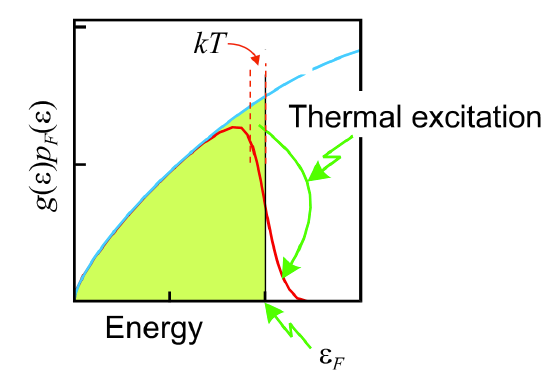
\includegraphics[width=0.5\textwidth]{figs/fd-distribution.png}
    \caption{A plot of $g_F(\varepsilon)$ against $\varepsilon$ at temperature $T.$}
    \label{fig:electron-fd}
\end{figure}

Both electrons and phonons contribute to the solid heat capacity, giving a total dependence of 
\[
    C = \gamma T + \beta T^3. 
\]
under low temperatures. 

Note that we didn't consider the thermal smearing in Debye model. This is because phonons are bosons following Bose-Einstein distribution, so there can be any number of phonons occupying the same states. The density of states we saw in the phonon case are for the vibrational modes, which don't behave like particles and cannot be ``thermally excited'' to smear out the edges. 

It is probably more useful to just remember that 
\[
    \boxed{g_{\mathrm{ph} }(\omega) \propto \omega ^{2}, \quad 
    g_{\mathrm{el, 3D} }(\omega ) \propto \omega ^{1 / 2}}
\]

\subsection{Electrical and optical properties of metals}
The free electron models allow us to predict various properties of \textit{metals}. For example, the internal energy per electron is
\[
    \expval{U} = \frac{\int_{0}^{\varepsilon_F} \varepsilon g(\varepsilon ) \,\mathrm{d}\varepsilon  }{\int_{0}^{\varepsilon_F} g(\varepsilon ) \,\mathrm{d}\varepsilon  } = \frac{3}{2}\varepsilon_F,
\]
giving the Pauli pressure 
\[
    P = -\frac{\partial U}{\partial V} = \frac{2}{5}n \varepsilon_F
\]
and the \textit{\textbf{bulk modulus}}
\[
    B_T = -V \left( \frac{\partial p}{\partial V} \right)_{T} = \frac{2}{3}v \varepsilon_F. 
\]
This can account for most of the contribution to the bulk modulus in metals, even if it ignores correlation between electrons and long-range attraction from the lattice. 

Just like phonons, electrons can scatter from phonons or structural defects as well (ignoring electron-electron scattering which is complicated), giving an exponential decay in the average speed that acts like a drag force
\[
    \expval{v} = v_0 \exp(- t / \tau), 
\]
where $\tau$ is the expected time between collisions. 

Therefore, the net equation of motion in an EM field is 
\[
    \boxed{m^{*} \left(\frac{\mathrm{d}\mathbf{v} }{\mathrm{d}t} + \frac{\mathbf{v} }{\tau } \right) = - e \mathbf{E} - e \mathbf{v} \times \mathbf{B},} 
\]
where $m^{*}$ is the effective mass accounting for lattice interaction and the magnetic force can often be neglected. This gives a steady-state drift velocity and hence the \textit{\textbf{electrical conductivity}} as 
\[
    \sigma  = \frac{n e^{2} \tau }{m^*} \coloneqq n e \mu. 
\]
When the damping is ignored (at high $\omega$), the equation of motion just becomes that of a free plasma, with a \textit{\textbf{dielectric constant}} $\epsilon(\omega ) = 1 / \omega_{p^{2} } / \omega ^{2}. $ This explains the variation of optical reflectivity as a function of $\omega$ in metals. 

Applying a constant $\mathbf{E} $ field essentially translates the Fermi sphere. Both phonon (high $q$ but low $\varepsilon,$ $40\mathrm{meV} \ll 5\mathrm{eV} $)and structural scattering changes the direction of the wavevector significantly, but not the magnitude. Therefore, the electrons in the Fermi sphere will be randomly scattered onto other parts on the surface of the sphere, with the higher $\left\vert k \right\vert $ states being scattered more, allowing the Fermi sphere to come to equilibrium at the drift velocity. 

At low temperatures, the structural defects dominates, so $\tau$ tends to sample-dependent constants, whereas at high temperatures, we expect the phonon scattering to dominate, giving $\tau \propto 1/T.$ Therefore, \underline{resistivity tends to a constant at low $T$ and is $\propto T$ for high $T$.}

Thermal conductivity can be determined from the usual \(\kappa  = \frac{1}{3} C_{el} \expval{c} l,\) where $\expval{c}$ is the average speed at the Fermi edge and $l = v_F \tau.$ It can be shown that good thermal conductors are usually also good electric conductors, since
\[
    \frac{\kappa }{\sigma } \propto T
\]
from the free electron model. This shows good agreement with experiments. Thermal conductivity of pure metals are hundreds times larger than those in insulators. 

The sign of quantum hall effects cannot always be accurately predicted by the model, marking its limitations.

\section{Nearly free electron model}
\subsection{The theory}
The free electron model fails to account for the sign of the hall coefficient, as it doesn't include the periodicity of a lattice (the electrons Hamiltonian only has the kinetic term). A solid can be better modelled with a periodic potential with Fourier series
\[
    V(x) = \sum_{p=-\infty }^{\infty} V_p \cos(p G_1 x). 
\]
When the potential is weak, we could use a perturbative approach to investigate its expansion coefficients in the eigenstates of the free electron (plane waves).

From the translational symmetry \(\left\vert \psi(x+a) \right\vert = \left\vert \psi(x) \right\vert \), the Bloch's theorem allows us to write the wavefunction as 
\[
    \psi_{\mathbf{k}} (\mathbf{r}) = u_{\mathbf{k}}(\mathbf{r}) e^{i \mathbf{k} \cdot \mathbf{r}}, 
\] 
where $\mathbf{k}$ is the free electron wavevector and $u_k{\mathbf{r}}$ is a periodic function, and the wavefunction can be in turn expanded into the Fourier series
\[
    \boxed{
        \psi_k(x) = \sum_{n=-\infty }^{\infty} C_{k,n} \ket{\phi_{k,n}}, \quad 
        \ket{\phi_{k,n}} \propto e^{i (k + n G_1) x}, 
    }
\]
where the basis functions are discrete values of the free electron scattering states (plane waves) satisfying the periodicity of the lattice. Here $k$ is best interpreted as the crystal momentum of the electron and comes directly from Bloch's theorem. From the perturbation theory, the contribution from various basis states depend on the energy difference to the central state $n=0.$ To first order, we could approximate solution as a linear combination of the two eigenstates with the nearest energy $\ket{k,0}$ and $\ket{k,-1}:$
\[
    \psi_K(x) = C_{k,0} \ket{\phi_{k,0}} = C_{k,-1} \ket{\phi_{k,-1}}. 
\]

For small values of $k,$ the contribution from $\ket{\phi_{k,0}}$ and the energy is close to the free dispersion curve. It is only near the zone boundary does the potential starts to play a role, which we can analyse from degenerate perturbation theory. 

In the finite eigenspace spanned by $\ket{\psi_{k,n}},$ the Schrodinger's equation for 
\[
    \psi(x) = \sum_{n=-\infty }^{\infty } C_{k,n} \ket{\phi_{k,n}(x)}
\]
can be rewritten as a eigenvalue equation on the expansion coefficients
\[
    \mathbf{\underline{H}} \mathbf{C} = \varepsilon \mathbf{C},  
\]
where the matrix elements of $\mathbf{H}$ in the eigenspace can be evaluated as a sum of delta functions
\[
    H_{nm} = \frac{\hbar^{2} (m G_1 + k)^{2} }{2m_e}\delta_{n,m} + \sum_{p=1}^{\infty} \frac{V_p}{2}(\delta_{n,m+p} + \delta_{n,m-p}). 
\]
The kinetic energy of the plane wave contributes to the diagonal entries and the Fourier components of $V(x)$ contribute to the off-diagonal elements. In the two-wave approximation, this becomes a matrix equation with contribution from the $V_1.$ 

In general, there would be continuous energy bands followed by forbidden band gaps. The widths of the n-th band gaps will be $V_n.$ This can also be regarded as backfolding of the free electron dispersion curve into the first Brillouin zone and lifting the degeneracies at the zone boundaries due to lattice interactions. For a electrons, higher-order zones will have a larger energy range and higher-order gaps will be narrower. This is due to the quadratic dispersion curve of electrons. This is in sharp contrast with the phonons with increasing band gaps and decreasing band widths, as shown in Fig.\ref{fig:band-structure}.
\begin{figure}[ht]
    \centering
    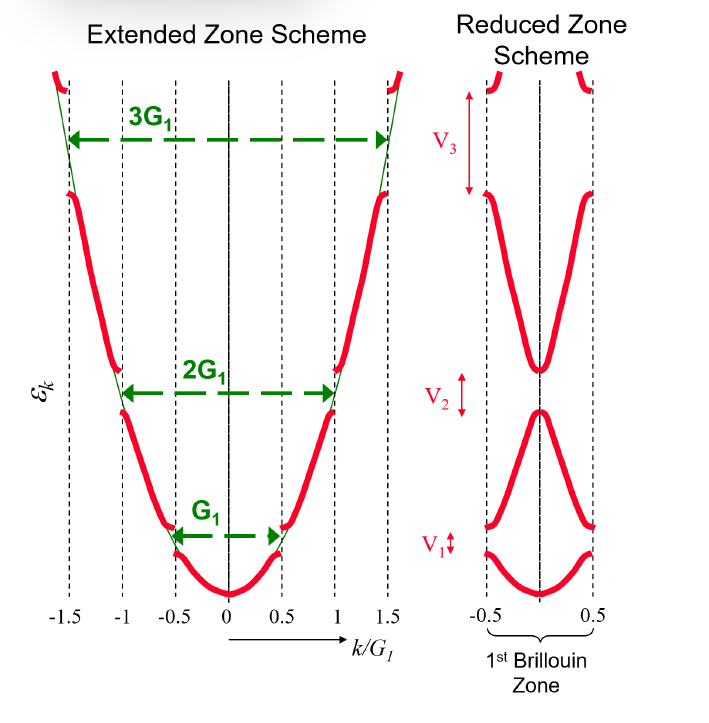
\includegraphics[width=0.5\textwidth]{figs/nfe-band-gaps.png}
    \caption{Band structures in the nearly free electron model.}
    \label{fig:band-structure}
\end{figure}
\section{Semiconductors}
\end{document}